\documentclass[12pt]{article}
\usepackage{graphicx}
\usepackage{wrapfig}
\usepackage{subcaption}
\usepackage[margin=1in]{geometry}
\usepackage{amsmath} % or simply amstext
\usepackage{amssymb}
\usepackage{siunitx}
\usepackage{booktabs}
\usepackage[export]{adjustbox}
\newcommand{\angstrom}{\textup{\AA}}
\newcommand{\colormap}{jet}  % colorbar to use
\usepackage{cleveref}
\usepackage{booktabs}
\usepackage{float}
\usepackage{indentfirst}
\usepackage[labelfont=bf]{caption}
\usepackage{titlesec}
\usepackage{setspace}
\usepackage{xcolor}
\usepackage{float}

\singlespacing
\setlength{\parindent}{5ex}
\setlength{\parskip}{0.05in}

\titlespacing{\section}{0pt}{\parskip}{-\parskip}
% \titlespacing{\subsection}{0pt}{\parskip}{-\parskip}
\titleformat*{\section}{\small\bfseries}
\titleformat*{\subsection}{\bfseries}

\title{Forecasting PSCO Energy Demand}
\author{Nate Schwindt}
\date{April 30, 2022}

\begin{document}
% \vspace{-50pt}
\maketitle

%%%%%%%%%%%%%%%%%%%%%%%%%%%%%%%%%%%%%%%%%%%%%%%%%%%%%%%%%%%%%%%%%%%%%%%%%%%
\section*{Introduction} 
%%%%%%%%%%%%%%%%%%%%%%%%%%%%%%%%%%%%%%%%%%%%%%%%%%%%%%%%%%%%%%%%%%%%%%%%%%%

The US Energy Information Administration (EIA) began collecting hourly energy demand data for the lower 48 states in 2015. These data are reported under EIA Form-930. According to the EIA-930, Hourly and Daily Balancing Authority Operations Report, the purpose of the data collection is "to provide basic operating information about the nation's electric power system on a current and historical basis" for use by many parties including the general public, policymakers, and industry partners. All electricity balancing authorities (BAs) are required to submit hourly integrated values in megawatts by hour. However, each BA performs its own data collection with its own procedures for anomalous values. The BA responsible for reporting Colorado energy demand is the Public Service Company of Colorado (PSCO). Here, I have gathered PSCO energy demand data from the EIA API and developed a model to forecast the hourly energy demand.

Reliable methods for predicting energy demands are necessary not only to ensure we are productive and happy now but also that we can remain so in a sustainable way. PSCO is responsible for generation, purchase, transmission, and distribution of electricity in Colorado, and therefore, it is responsible for knowing how much energy is needed and how to get it to Coloradans. Reliable forecasts provide time to prepare for scheduled outages, and they can inform the highest priority areas for unplanned power outages. With a growing climate crisis and depleting natural resources, we must know our energy needs in the future so we can develop new ways to generate, distribute, and use electricity. Either a gross underestimate or overestimate of energy demand will lead to an unsustainable future.

The forecasting strategy presented here is as follows:
\begin{enumerate}
    \item Data acquisition through freely-accessible online resources
    \item Data preprocessing to remove outliers, fill missing data, and cleanly scale the data
    \item Regression modeling to remove most of the trend, seasonality, and temperature dependence
    \item Seasonal ARIMA modeling to forecast future energy demand
\end{enumerate}

%%%%%%%%%%%%%%%%%%%%%%%%%%%%%%%%%%%%%%%%%%%%%%%%%%%%%%%%%%%%%%%%%%%%%%%%%%%
\section*{Data Acquisition} 
%%%%%%%%%%%%%%%%%%%%%%%%%%%%%%%%%%%%%%%%%%%%%%%%%%%%%%%%%%%%%%%%%%%%%%%%%%%

The energy demand for Colorado is obtained from the EIA API under Category 3389994 using the Python package \texttt{eiapy}. \texttt{eiapy} interacts with the EIA API in order to access its Open Data and returns the data and corresponding metadata in easily accessible Python classes. Energy demand is correlated with temperature, since heating and cooling systems require a large electricity input. Temperature data is obtained from Meteostat. Meteostat provides free hourly weather and climate data from the National Oceanic and Atmospheric Administration, and the data are accessible through a convenient Python library \texttt{meteostat}. I hypothesized that energy demand is more strongly correlated with temperature in highly populated areas than with temperature in sparsely populated areas. Therefore, I weighted temperature by population percentage for cities across Colorado. The city and population data are from \texttt{simplemaps.com}, which reports data from the U.S. Geological Survey and U.S. Census Bureau for over 108,000 cities in the U.S. The method for weighting temperature is presented in the following section. 

%%%%%%%%%%%%%%%%%%%%%%%%%%%%%%%%%%%%%%%%%%%%%%%%%%%%%%%%%%%%%%%%%%%%%%%%%%%
\section*{Data Preprocessing} 
%%%%%%%%%%%%%%%%%%%%%%%%%%%%%%%%%%%%%%%%%%%%%%%%%%%%%%%%%%%%%%%%%%%%%%%%%%%

\begin{figure}[h]
    \centering
    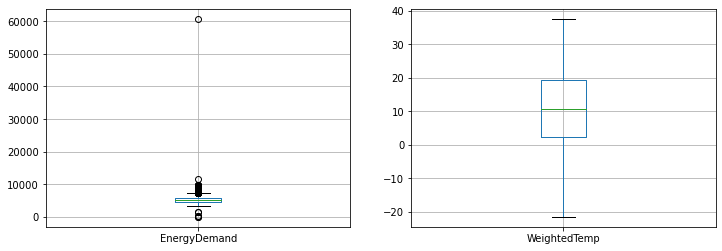
\includegraphics[width=0.9\textwidth]{figures/boxplots.png}
    \caption{Boxplots of the energy demand (left) and weighted temperature (right). The energy demand shows many outliers above and below the interquartile range. The weighted temperature does not show any outliers.}
    \label{fig:boxplots}
\end{figure}

Meteostat can provide hourly weather data for any latitude, longitude coordinate by interpolating weather data of the nearest weather stations. I select the top 20 most populated cities in Colorado and collected weather data for each of their coordinates. I fill missing values in each city's temperature time series through linear interpolation. To weight these temperature data by population, I determine each cities population percentage and weight the hourly temperature of each city by its population percentage. Equation \ref{eq:weighted_temp} shows the population-weighted temperature for one timestep $t$. 

\begin{equation}
    \text{WeightedTemp}(t) = T_1(t) \frac{p_1}{p_{tot}} + T_2(t) \frac{p_2}{p_{tot}} + ... + T_{20}(t) \frac{p_{20}}{p_{tot}}
    \label{eq:weighted_temp}
\end{equation}

$T_i(t)$ and $p_i$ are the temperature at time $t$ and population for city $i$, respectively. $p_{tot}$ is the total population of all 20 cities. This temperature weighting is equivalent to a center of mass calculation where temperature is equivalent to position and population is equivalent to population.

Figure \ref{fig:boxplots} shows boxplots for the energy demand and the weighted temperature data. The energy demand has clear outliers, but the weighted temperature does not. The interquartile range (IQR) test is applied to the energy demand time series to remove outliers. The IQR is defined as the range from the first quartile to the third quartile, and the IQR test removes values that are outside the quartiles by more than 150\% of the IQR. I replace the outliers by linear interpolation in order to have a complete time series with no missing values.

\begin{figure}[h!]
    \centering
    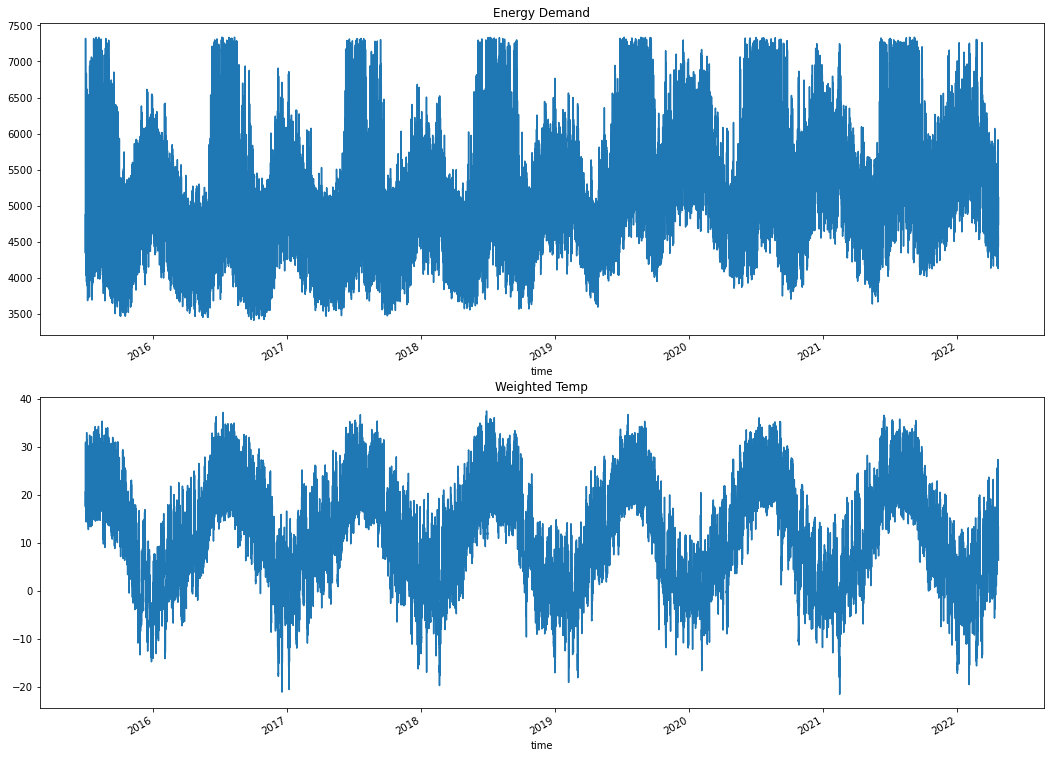
\includegraphics[width=0.75\textwidth]{figures/cleaned_data.png}
    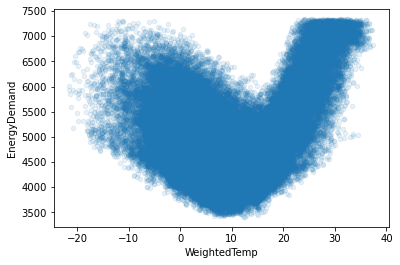
\includegraphics[width=0.5\textwidth]{figures/power_vs_wtemp.png}
    \caption{The top two figures are the clean energy demand and weighted temperature, respectively. Both show obvious seasonality and no clear outliers. The final plot is the energy against weighted temperature, which appears to be roughly quadratic.}
    \label{fig:cleaned_data}
\end{figure}

Figure \ref{fig:cleaned_data} shows the energy demand and weighted temperature after filling missing data and removing outliers. The time series appear to have many seasonal frequencies and some trend. Figure \ref{fig:cleaned_data} also shows energy demand plotted against weighted temperature, confirming the strong correlation discussed earlier. The relationship appears to be roughly quadratic, which informs the regression modeling choice.

The periodogram in Figure \ref{fig:periodogram} shows the most prominent seasonality in the energy demand, which is necessary for harmonic regression modeling described in the following section. I list the frequencies and their corresponding periods with the highest spectral densities in order to determine the most important harmonics. The most prominent periods include 24 hours, 4266 hours, 12 hours, 168 hours, and 84 hours. These periods roughly correspond to daily, semi-daily, weekly, semi-weekly, and annually. Finally, the energy demand and the weighted temperature are scaled to 0 mean and unit variance. Standardized scaling improves the performance of regression modeling, and it ensures the model captures the relationships between features of different units.

\begin{figure}[h!]
    \centering
    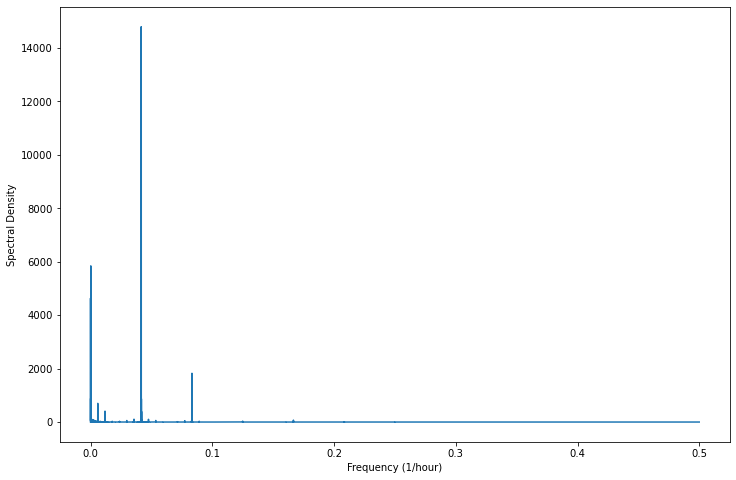
\includegraphics[width=0.5\textwidth]{figures/periodogram.png}
    \caption{Periodogram of the energy demand used to determine the most prominent periods.}
    \label{fig:periodogram}
\end{figure}

%%%%%%%%%%%%%%%%%%%%%%%%%%%%%%%%%%%%%%%%%%%%%%%%%%%%%%%%%%%%%%%%%%%%%%%%%%%
\section*{Modeling and Forecasting} 
%%%%%%%%%%%%%%%%%%%%%%%%%%%%%%%%%%%%%%%%%%%%%%%%%%%%%%%%%%%%%%%%%%%%%%%%%%%

The model presented here is an additive model for trend, seasonality, temperature dependence, and residuals. This relationship is shown in Equation \ref{eq:model}.

\begin{equation}
    \text{EnergyDemand} = m(t) + s(t) + f(T) + w(t)
    \label{eq:model}
\end{equation}

Here, $m(t)$ is the trend, $s(t)$ is the seasonality, $f(T)$ is the temperature dependence, and $w(t)$ is the residuals. The simple additive model is easy to interpret and can capture much of the variance in the data. Additionally, I model the residuals using an ARIMA process, which should capture any remaining variance in the data. I use ridge regression to fit linear parameters for each of these components. Ridge regression is simple and includes a penalty for the number of coefficients. Ridge regression finds the coefficients $\bf{\beta}$ that minimize

\begin{equation*}
    \sum{(y_i - \bf{\beta}x_i)^2} + \lambda \sum{\beta_k}^2 
\end{equation*}

\begin{figure}[h]
    \centering
    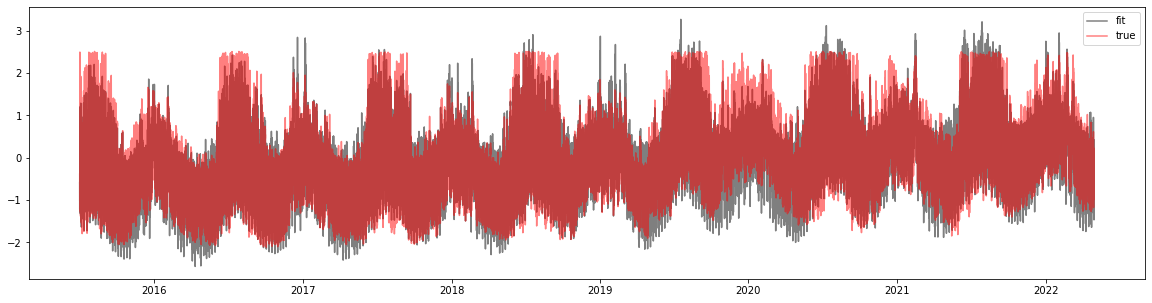
\includegraphics[width=0.8\textwidth]{figures/model_fit.png}
    \caption{The estimate of energy demand (blue) and the historical energy demand (black).}
    \label{fig:model_fit}
\end{figure}

I model the trend component as a simple linear trend, the seasonal component as a sum of harmonics, and the temperature dependence as a quadratic. I iteratively determined the best choice of features by looking at model mean squared error. Beginning with only a linear temperature dependence, the mean squared error was 0.9460 using a 5-fold time series cross validation. The best model I found with the ridge regression framework had a mean squared error of 0.1620, and Figure \ref{fig:model_fit} shows the fit in blue and the data in black. Equation \ref{eq:final_model} shows the model of energy demand. 

\begin{align} \label{eq:final_model}
\begin{split}
    \text{EnergyDemand} &= \beta_0 + \beta_1 t + \beta_2 T + \beta_3 T^2 \\
    &+ \beta_4 \sin \left( \frac{2 \pi t}{12} \right) + \beta_5 \cos \left( \frac{2 \pi t}{12} \right) \\
    &+\beta_6 \sin \left( \frac{2 \pi t}{24} \right) + \beta_7 \cos \left( \frac{2 \pi t}{24} \right) \\
    &+ \beta_8 \sin \left( \frac{2 \pi t}{84} \right) + \beta_9 \cos \left( \frac{2 \pi t}{84} \right) \\
    &+ \beta_{10} \sin \left( \frac{2 \pi t}{168} \right) + \beta_{11} \cos \left( \frac{2 \pi t}{168} \right) \\
    &+ \beta_{12} \sin \left( \frac{2 \pi t}{4380} \right) + \beta_{13} \cos \left( \frac{2 \pi t}{4380} \right) \\
    &+ \beta_{14} \sin \left( \frac{2 \pi t}{8760} \right) + \beta_{15} \cos \left( \frac{2 \pi t}{8760} \right) \\
    &+ w(t)
\end{split}
\end{align}

Finally, I model $w(t)$ with an ARIMA model to be added back to the estimate for energy demand. Figure \ref{fig:residuals} shows the residuals from the energy demand model and their autocorrelation function. The residuals appear to still have daily seasonality, so I include a seasonality component in the ARIMA model (i.e. SARIMA model). I fit the SARIMA model and choose the model with the best AIC. The best model is an ARIMA(4,1,0)(2,0,0) with 24 hour periodicity, where (2,0,0) corresponds with the seasonality coefficients. The AIC for this model is -84,250, which is smaller than all models $0 < p <= 5$, $0 < q <=5$, $d = 1$, $0 < P <= 2$, $0 < Q <= 2$, and $D = 1$.

\begin{figure}[h]
    \centering
    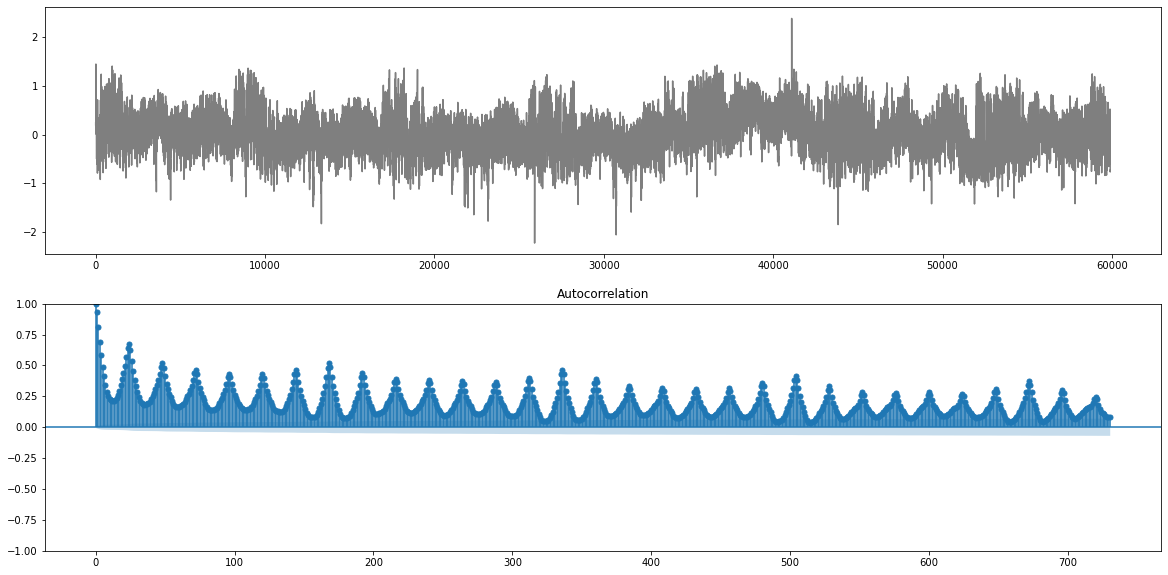
\includegraphics[width=0.8\textwidth]{figures/residuals.png}
    \caption{The residuals (top) and their autocorrelation function (bottom). The ACF indicates there is still daily seasonality.}
    \label{fig:residuals}
\end{figure}


%%%%%%%%%%%%%%%%%%%%%%%%%%%%%%%%%%%%%%%%%%%%%%%%%%%%%%%%%%%%%%%%%%%%%%%%%%%
\section*{Conclusions}
%%%%%%%%%%%%%%%%%%%%%%%%%%%%%%%%%%%%%%%%%%%%%%%%%%%%%%%%%%%%%%%%%%%%%%%%%%%

The model predicts the energy demand from 5-6 PM on May 1st to be 5036.9 $\pm$ 1122.4 megawatt hours. Figure \ref{fig:forecast} shows the final forecast for energy demand through May 1st with the historical data for the previous week. The confidence intervals (shown as blue dotted lines) appear reasonable for the next few hours but quickly span the full possible range of energy demand values after 24 hours. The model presented here appears to make a reasonable prediction as indicated by narrow confidence intervals, low AIC in the ARIMA model, and moderate mean squared error in the regression model. However, this model is simple and can be improved. Possible improvements to the regression model are to use more advanced modeling techniques that could better capture the variance in the data. In particular, the weighted temperature dependence would require a much more rigorous model search, since a quadratic model is not very appropriate. In the future, a more accurate regression method would be preferred, such as a gradient boosting tree. Other more powerful methods that could be applied include support vector machines or deep neural nets. Both of these methods are more computationally intensive, but they are very good at identifying patterns in the data. These methods would not need predefined models for temperature dependence and seasonality harmonics. These choices are limitations of my model, as I chose specific, limited harmonics and a quadratic dependence on temperature that I expected in the data. Improvements to the ARIMA model include a fuller parameter search and better seasonality removal. The ARIMA model presented here tests only one differencing parameter $d=1$ and limited values for $p$ and $q$. A larger parameter search could reveal a better ARIMA model.

\begin{figure}[h]
    \centering
    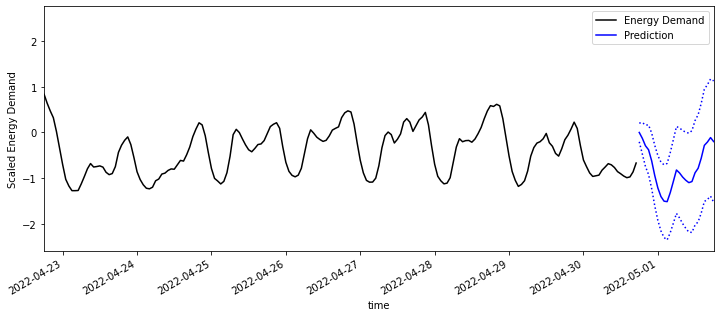
\includegraphics[width=0.6\textwidth]{figures/forecast.png}
    \caption{The 24-hour forecast for PSCO energy demand. Historical data for the previous week is shown in black, and the model prediction with confidence intervals from the ARIMA model fit shown in blue.}
    \label{fig:forecast}
\end{figure}

\clearpage
\pagebreak

\end{document}